Let there exist a particular origin-destination pair $o-d$ with a
CMS near $o$. There are two paths that can be taken to go between
$o$ and $d$, and the CMS will post a message addressed to those
traveling $o-d$ to take route 1 over 2, with some percentage of those drivers complying. For simplicity, we assume instead that our control is a split
ratio $\beta$ for the $o-d$ drivers at the point of the CMS.

In addition, there an arbitrary
number of additional sources and sinks, but the CMS only targets $o-d$.
The additional sources and sinks may have viable paths through both
$o$ and $d$, complicating the determination of demand between $o-d$
specifically. The Eulerian flow is known over each link in the network,
over all discrete time steps.

We cannot determine which flows belong to $o-d$ drivers versus all
others from this problem setup due to the non-uniqueness of OD-estimation
problem. But if we assume we know the path flows of just taking $o-d$,
then source flows and split ratios may be determined for the other
OD's. From this assumption of data (path flows for $o-d$, source
flows and split ratios for all others), one can use the Piccoli class-based
forward simulation framework as the flow model, where the classes
are controllable $o-d$ flows and uncontrollable flows from all other
OD pairs. This is illustrated in Figure~\ref{fig:Diagram-of-network}.
\begin{wrapfigure}{r}{0.2\textwidth}
\begin{centering}
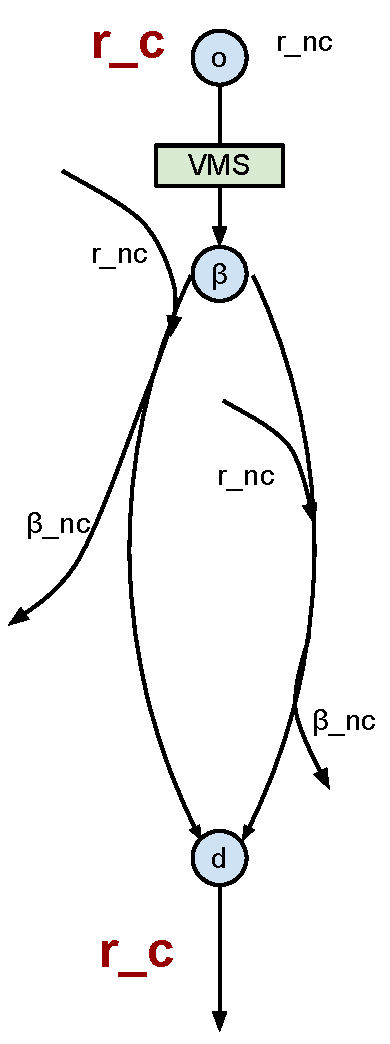
\includegraphics[scale=0.4]{NetworkForCMS}
\par\end{centering}

\caption{Diagram of network under consideration\label{fig:Diagram-of-network}. $r_c, r_{nc}$ are the flows in for controllable and non-controllable drivers. $\beta_{nc}$ are the estimated split ratios for the non-controllable, which can be determined after estimating initial controllable flows on the left and right paths.}
\end{wrapfigure}


One special case of this set of assumptions is rerouting drivers not
attending a popular event, while those attending have no rerouting
options.

One approach is to determine an upper and lower bound on the demands
on routes 1 and 2 for $o-d$. Then we take a robust optimization approach
to create an optimal split-ratio policy $\beta^{*}$ for the worst
case \emph{actual} demand on $o-d$. It is unclear how robust optimization
exactly fits within the adjoint framework, but there is previous work
in this area.

Another approach seeks to \emph{learn} the $o-d$ demands at the CMS
location from a feedback-loop approach. After witnessing how the split
ratio at the CMS changes due to some displayed split ratio, one can
estimate the population of drivers that responded to the message from
all drivers on the network.

Both of these approaches attempt to deal with the fact that we do
not have enough information to do rerouting at the CMS and still guarantee
that the original demand profiles would be satisfied. Any approach
that seeks to do rerouting on Eulerian data would have to embrace
such methods in some form.
